%\section{\KSe}
%\label{sec:KSe}

The \KS\ [henceforth KS] system was derived by
Kuramoto and Tsuzuki\rf{ku} as a phase equation for
reaction-diffusion systems described by Complex Ginzburg-Landau
equation and independently by Sivashinsky\rf{siv} to describe
instabilities in laminar flame fronts. It also appears
in a variety of contexts including thin falling
films\rf{BenKS66,LinKS74}, interfacial instabilities between
concurrent viscous fluids, drift waves in plasmas.
    \ES{citations needed.}
% For an instructive derivation from Complex Ginzburg-Landau
% equation \cf~\rf{}.

Our motivation for its study is that it is one of the simplest
nonlinear PDEs that exhibit spatiotemporally chaotic behavior.
Moreover the dynamics in the chaotic regime are interesting in
their own right.

 In the formulation
adopted here, the time evolution of the `flame front velocity'
$u=u(x,t)$ %on a periodic domain $u(x,t) = u(x+L,t)$
is given by
\beq
  u_t = F(u) = -{\textstyle\frac{1}{2}}(u^2)_x-u_{xx}-u_{xxxx}
    \,,\qquad   x \in [-L/2,L/2]
    \,,
\ee{ks}
with appropriate boundary conditions, as discussed in \refsect{sec:KSbc}.
Here $t \geq 0$ is the time, and $x$ is the spatial coordinate.
The subscripts $x$ and $t$ denote partial derivatives with respect to
$x$ and $t$.

\subsection{Boundary conditions and system size}
\label{sec:KSbc}

Ideally when one is interested in studying PDEs that exhibit spatiotemporal chaos one
would like to work in a system of infinite spatial extend, \ie\ in the limit $L\rightarrow\infty$.
Although solutions of KS equations in this limit have appeared, \cf for example \refrefs{hooper_travelling_1988,feng_multiplicity_2004}\ES{More citations needed. Kevrekidis \etal\
mention criticism of periodic BC, but they give no reference.}, it is
more convenient, both computationally and theoretically, to work with periodic boundary conditions
\beq
  u(x,t) = u(x+L,t)\,,
 \label{eq:KSper}
\eeq
and this is the usual choice in the literature and the one followed in this thesis.
% The justification in terms of the physics
% of the problem is that we focus our attention to a small part of a larger system,
% far away from the boundaries. Further
Justification of this choice will be given
in \refsect{sec:KSeSymm}, in conjunction with the discussion of the symmetries of the system.

Another common choice of boundary conditions is
\beq
  u(0,t) = u(L,t)=0\,,
 \label{eq:KSodd}
\eeq
which restricts the system to the subspace of odd functions. This choice will also be discussed
in \refsect{sec:KSeSymm}.

In what follows
we shall state results of all calculations either in units of the system size $L$
or the `dimensionless system size' $\tildeL=L/2\pi$.
All numerical results presented in this thesis
are for $\tildeL=22/2\pi = 3.5014\ldots$, unless otherwise
noted. The specific choice leads to a system that is just ``chaotic'' enough
to have interesting dynamics, \cf \refsect{sec:KSlit}, but is not in the spatio-temporally chaotic
regime, therefore it is still rather tractable and we can use it as a test bed for
continuous symmetry reduction and a dynamical systems approach.


\subsection{Symmetries of \KS\ system}
\label{sec:KSeSymm}

In an unbounded domain, $x\in(-\infty,\infty)$, KS equation is equivariant
under the action of the non-compact Euclidean group $\En{1}$:
If $u(x,t)$ is a solution, then
$\Shift({\shift})\, u(x,t) = u(x+\shift,t)$
is an equivalent solution for any shift
$\shift\in\Rls{}$, as is the reflection (`parity' or `inversion')
\beq
    \Refl \, u(x) = -u(-x)
\,.
\ee{KSparity}

Imposing periodic boundary conditions we restrict attention to the subspace 
$[-L,L]$ in which only the compact subgroup \On{2} of \En{1} acts by:
\beq
	\Shift_{\shift/L}\, u(x,t) = u(x+\shift,t)\,,\qquad \shift\in\left[-L/2,L/2\right]	
	\label{KSshift}
\eeq
and reflections \refeq{KSparity}. Here we use subscript
notation for shifts to differentiate with the case of \En{1}.
Moreover, we only consider perturbations within this subspace,
\ie\ we do not consider subharmonic perturbations. The system
size $L$ affects the representation of \On{2}, \cf
\refsect{sec:fourKS}. \ES{This statement needs to be checked:
An important fact is that the isotropy subgroups of \En{1} (of
\En{n} in general) are all compact subgroups, if the action is
proper, see for example \refref{ChossLaut00}. Thus the
equivariant bifurcation structure as $L$ increases is not
affected, at least as long as we are not in the
spatio-temporally chaotic regime, when the spectrum of
stability eigenvalues becomes quasi-continuous.} Reflection
generates the dihedral subgroup $\Dn{1} = \{1, \Refl\}$ of
$\On{2}$. Boundary conditions \refeq{eq:KSodd} restrict the
system to \Fix{\Dn{1}} and thus in that case symmetry \Dn{1}
is impossed to all solutions. To avoid technical difficulties
associated with the action of \On{2} on an infinite dimensional
space we will discuss the isotropy subgroups of \On{2} in
\refsect{sec:ksIso}, after we truncate \refeq{expan} to finite
order.


The KS equation is also Galilean invariant: if $u(x,t)$ is a solution,
then $u(x -ct,t) -c $, with $c$ an arbitrary constant
speed, is also a solution. As one can verify by integrating \refeq{ks} with
respect to $x$ over the periodic domain $[-L/2,L/2]$ the quantity
 $\int_{-L/2}^{L/2} u\,dx$
is conserved and we can, without loss of generality, set it equal to zero. This corresponds
to the choice $c=0$, therefore eliminating Galilean invariance.


% $G$, the group of actions $ g \in G $ on a
% \statesp\ (reflections, translations, \etc) is a symmetry of the KS
% flow \refeq{ks} if $g\,u_t = F(g\,u)$.

% The KS equation is time translationally invariant, and space translationally invariant
% on a periodic domain under
% the 1-parameter group of
% $O(2): \{\Shift_{\shift/L},\Refl \}$.
% If $u(x,t)$ is a solution, then
% $\Shift_{\shift/L}\, u(x,t) = u(x+\shift,t)$
% is an equivalent solution for any shift
% $-L/2 < \shift \leq L/2$,
% as is the
% reflection (`parity' or `inversion')
% \beq
%     \Refl \, u(x) = -u(-x)
% \,.
% \ee{KSparity}



\subsection{Fourier space}
\label{sec:fourKS}

\On{2} equivariance makes it convenient to work in Fourier space,
\beq
  u(x,t)=\sum_{k=-\infty}^{+\infty} a_k (t) e^{ i k x /\tildeL }
\,,
\ee{eq:ksexp}
with the $1$-dimensional PDE \refeq{ks}
replaced by an infinite set of
ODEs for the complex Fourier coefficients $a_k(t)$:
\beq
\dot{a}_k= \pVeloc_k(a)
     = ( q_k^2 - q_k^4 )\, a_k
    - i \frac{q_k}{2} \sum_{m=-\infty}^{+\infty} a_m a_{k-m}
\,,
\ee{expan}
where $q_k = k/\tildeL$.
Since $u(x,t)$ is real, $a_k=a_{-k}^\ast$, and we can replace the
sum by a $k > 0$ sum. Note that $\dot{a}_0=0$ in
 \refeq{expan} as a result of Galilean invariance and $a_0$ is a conserved quantity
 fixed to $a_0=0$ by the condition $\int_{-L/2}^{L/2} u\,dx$=0.
In the Fourier basis \On{2} acts absolutely irreducibly on each complex plane
$\left(\Re(a_k),\Im(a_k)\right)$ and the linear part of \refeq{expan} is conveniently
diagonalized. Indeed, the translation operator action on the Fourier coefficients \refeq{eq:ksexp},
represented here by a complex valued vector
$a = \{a_k\in\mathbb{C}\,|\,k = 1, 2, \ldots\}$, is given by
\beq
  \Shift_{\shift/L}\, a = \mathbf{g}(\shift) \, a \,,
  \label{eq:shiftF}
\eeq
where $\mathbf{g}(\shift) = \mathrm{diag}( e^{i q_k\, \shift} )$ is a complex
valued diagonal matrix, which amounts to the $k$-th mode complex plane
rotation by an angle $k\, \shift /\tildeL$.  The reflection acts on
the Fourier coefficients by complex conjugation and a change of sign,
\beq
  \Refl \, a = -a^\ast
\,.
\label{eq:FModInvSymm}
\eeq

We can now justify the choice of boundary conditions and system size. With periodic boundary conditions
we expect to find traveling wave and modulated amplitude traveling wave solutions which
are the objects that we want to understand how they fit into the framework of earlier
approaches \rf{Christiansen97,LanThesis,lanCvit07}. Moreover,
we have observed in numerical simulations that $L=22$ is just after the onset of chaos while still
not spatio-temporally chaotic. As we will see in \refchap{chap:kseStSp}, many of the invariant objects
(\eqva, \reqva, {\po s}, {\rpo s}) have more than one unstable eigenspaces, a situation that has not
been dealt with in the above references and which very often occurs in the studies of \pCf\ in 
\refrefs{GHCW07,HGC08,GHCV08,HalcrowThesis}. Nevertheless the system of this size seems to remain
within reach of a dynamical description, see \refchaps{chap:kseStSp}{chap:kseRedStSp}.


\ES{This is from my first year KS special problem, perhaps some parts are usable:
Some qualitative comments about the KS equation can now be easily
given in view of \refeq{expan}. The linear behavior of the system
depends on the sign of the quantity $k^2- \left(2\pi/L\right)  k^4$.
For a sufficiently large system, the first few values of $k$ yield $k^2- \left(2\pi/L\right)
k^4>0$ or $k<\sqrt{L/2\pi}$ and the corresponding Fourier components grow exponentially
with time (unstable components). In other words the anti-diffusion
term in \refeq{eq:KS} (resulting in the term $\sim k^2$ in
\refeq{eq:Fcoef}) dominates over the dissipation term (resulting in
$\sim k^4$ in \refeq{eq:Fcoef}).  On the other hand there are infinitely many larger
wavenumber components with $k>\sqrt{L/2\pi}$ for which the solutions
are bounded (stable components). The role of the bilinear term in
\refeq{eq:Fcoef} is then to excite the larger wavenumber components
while dissipating the smaller wavenumber ones. The result of this
competition is that the asymptotic dynamics of the system are
confined on a low dimensional attractor.}

\ES{Move elsewhere: Due to the hyperviscous damping $u_{xxxx}$, long time solutions of KS
equation are smooth, $a_k$ drop off fast
with $k$, and truncations of \refeq{expan} to $16 \leq N \leq 128$
terms yield accurate solutions for system sizes considered here.
Robustness of the long-time dynamics
of KS as a function of the number of Fourier modes kept in truncations
of \refeq{expan} is, however, a subtle issue.  Adding an extra mode to
a truncation of the system introduces a small perturbation in the
space of dynamical systems.  However, due to the lack of structural
stability both as a function of truncation $N$, and the system size
\tildeL, a small variation in a system parameter can (and often will)
throw the dynamics into a different asymptotic state.  For example,
asymptotic attractor which appears to be chaotic in a $N$-dimensional
\statesp\ truncation can collapse into an attractive cycle
for $(N\!+\!1)$-dimensions.}


\subsection{Truncation}

Dynamical \statesp\ representation of a PDE is $\infty$-dimensional,
but the KS flow is strongly contracting and its non-wondering set,
and, within it, the set of invariant solutions investigated here, is
embedded into a finite-dimensional inertial manifold\rf{FNSTks85} in
a non-trivial, nonlinear way. The existence of an inertial manifold for
KSe with both odd and periodic boundary conditions has been proved and
several bounds for its dimension have been found, \cf\ \refref{jolly_evaluating_2000} and references
therein. The best current bound in dimension of inertial manifold for KS
equation with periodic boundary condition is, to the authors knowledge,
given in \refrefs{Robinson_inertial_1994,jolly_evaluating_2000}: $O(L^{2.46})$ for $L\in[2\pi,6\pi]$.

The fact that the asymptotic dynamics lies on a finite
dimensional manifold justifies truncation of the infinite tower
of equations \refeq{expan} to finite order $N$. According to
the bound $O(L^{2.46})\simeq2000$ for $L=22$\ES{$L=22>6\pi$, so
it looks like their proof does not apply to our system if one
wants to be rigorous.} and we would expect to need even more
Fourier modes, since the Fourier basis is not directly
connected to coordinates on the inertial manifold of KSe and
would therefore be less optimal than an approach that
approximates such coordinates, for
example\rf{Jolly_approximate_1990,JRT01}.
Nevertheless such a bound seems rather inflated compared to
numerical simulations of the asymptotic dynamics that typically
require $O(10)-O(100)$ Fourier modes. In practice we keep
$16\leq N \leq 128$ Fourier modes in numerical simulations and
check the robustness of the results against increase of $N$.

\subsection{Isotropy lattice and invariant subspaces}
\label{sec:ksIso}

Let $N$ be the number of Fourier modes retained in \refeq{expan}
and observe that the action of $O(2)$
on \Rls{N} by \refeq{eq:shiftF} and \refeq{eq:FModInvSymm} is,
up to the minus sign in \refeq{eq:FModInvSymm}, identical
to the action \refeq{eq:O2stndrd} of \On{2} on \Clx{N} studied
in \refsect{sec:strata}.
The isotropy lattice remains unchanged but \fixedsp s of the dihedral subgroups are affected.
\Fixedsp\ of \Cn{q}, given by the condition
\beq
	a_k=0\ \mathrm{unless}\ k = q j\,,\ j=1,\ldots\lfloor n/q \rfloor\,,
	\label{eq:O2CqFix}
\eeq
remain unchanged but the \fixedsp s of the dihedral subgroups \Fix{\Dn{m}} are now given by the conditions
\bea
	a_k=0\ \mathrm{unless}\ k = m j\,,\ j=1,\ldots\lfloor n/m \rfloor\,, \\
	\Re(a_k)=0\ \mathrm{for}\ k=1,\ldots,n\,.
	\label{eq:O2ksDqFix}
\eea
In relation to physical space we observe that \Fix{\Dn{1}} is the subspace of antisymmetric functions $Re(z_k)=0,\, \forall k$ or $u(-x)=-u(x)$ while for the action \refeq{eq:O2stndrd} the corresponding
subspace would be that of symmetric functions.

\subsection{\Eqva\ and their bifurcations}

%%%%%%%%%%%%%%%%%%%%%%%%%%%%%%%%%%%%%%%%%%%%%%%%%%%%%%%%%%%%%%%%%%
\begin{figure}[ht]
\begin{center}
  (\textit{a})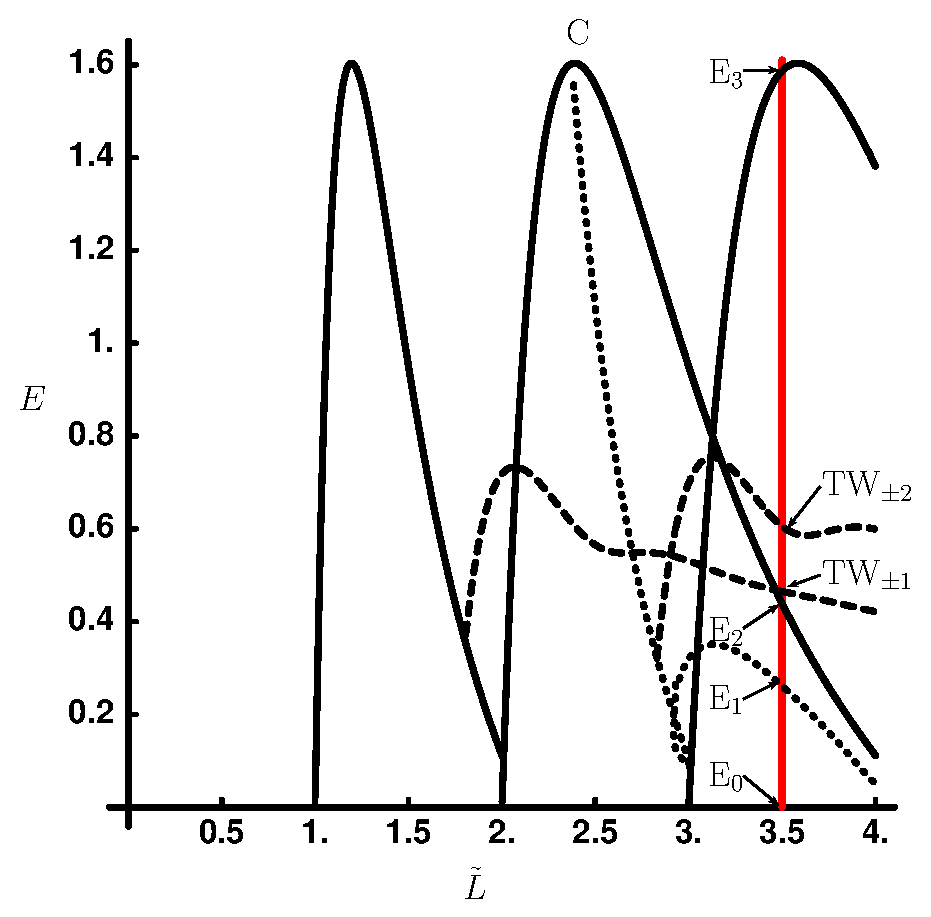
\includegraphics[width=0.5\textwidth]{../figs/ksBifDiag.eps}
\end{center}
\caption[KS steady state bifurcations]{
The energy \refeq{ksEnergy} of the \eqva\ and \reqva\ that
exist up to $L=22$, $\tildeL = 3.5014\ldots$, plotted as a function
of the system size $\tildeL = L/2\pi$ (additional \eqva, not present
at $L = 22$ are given in \refref{ksgreene88}). Solid curves denote
$n$-cell solutions \EQV{2} and \EQV{3}, dotted curves the GLMRT
\eqv\ \EQV{1},
and dashed curves the \reqva\ \REQV{\pm}{1} and \REQV{\pm}{2}.
The parameter $\alpha$ of \refrefs{KNSks90,ksgreene88} is
related to the system size by $\tildeL=\sqrt{\alpha/4}$.    }
\label{fig:ksBifDiag}
\end{figure}
%%%%%%%%%%%%%%%%%%%%%%%%%%%%%%%%%%%%%%%%%%%%%%%%%%%%%%%%%%%%%%%%

\Eqva\  (or the steady solutions)
are the fixed profile time-invariant solutions,
\beq
 u(x,t) = u_\stagn(x)
\,.
\ee{eqva}
Due to the translational symmetry,
the KS system also allows for
\reqva\ (traveling waves, rotating waves),
characterized by a fixed profile $u_\stagn(x)$
moving with constant speed $c$, {\ie}
\beq
 u(x,t) =  u_\stagn(x-ct)
\,.
\ee{reqva}
Here suffix ${}_\stagn$ labels a particular invariant solution.
Because of the reflection symmetry \refeq{KSparity},
the \reqva\ come in counter-traveling pairs
$u_\stagn(x-ct)$, $-u_\stagn(-x+ct)$.

The \reqv\ condition for the {\KS} PDE \refeq{ks}
is the ODE
\beq
{\textstyle\frac{1}{2}}(u^2)_x+u_{xx}+ u_{xxxx}=c \, u_x
\ee{KSeqvCond}
which can be analyzed as a dynamical system in its own right.
Integrating once we get
\beq
{\textstyle\frac{1}{2}}u^2 - c u + u_x + u_{xxx}=\expctE
\,.
\label{eq:stdks}
\eeq
This equation can be interpreted as a 3-dimen\-si\-on\-al dynamical system
with spatial coordinate $x$ playing the role of `time,'
and the integration constant \expctE\ can be interpreted as `energy,'
see \refsect{sec:energy}.

In the Fourier representation the \reqva\ time dependence is
\beq
 a_k(t) e^{-itc q_k} = a_k(0)
\,.
\ee{reqvaF}
Differentiating with respect to time, we obtain
the Fourier space version of the \reqv\ condition
\refeq{KSeqvCond},
\beq
 \pVeloc_k(a) - i q_k c a_k = 0
\,,
\ee{reqvCondF}
which we solve for (time independent) $a_k$ and $c$, see \refchap{chap:kseStSp}.

In a periodic box of size $L$
both \eqva\ and \reqva\ are  periodic solutions
embedded in 3-$d$ space, conveniently represented as loops in
$(u,u_x,u_{xx})$ space, see \reffig{f:KS22Equil}\,(\textit{d}).
In this representation the continuous translation symmetry
is automatic -- a rotation in the $[0,L]$ periodic domain only
moves the points along the loop. For an \eqv\ the points
are stationary in time; for \reqv\ they move in time, but in
either case, the loop remains invariant.
So we do not have the problem that we encounter in the Fourier
representation, where seen from the frame of one of the \eqva\
the rest trace out circles under the action of continuous symmetry
translations.

The  \eqva\ and \reqva\ of KS equation and their bifurcations have been
the object of extensive study and the literature is too hard to
exhaust. The results of main interest for this thesis can be
found in \refrefs{Mks86,laquey74,ksgreene88,KNSks90,AGHks89}.
Although the results were obtained by direct bifurcation
analysis rather than with use of methods of equivariant
bifurcation theory, the relation of bifurcations to \On{2}
symmetry has been recognized in the literature particularly in
\refrefs{KNSks90,AGHks89} The relation of the bifurcations
found numerically (and in some cases analytically) in
\refref{KNSks90} to the predictions of equivariant bifurcation
theory is discussed in Krupa\rf{Krupa90} but
without explicit calculations. In this section we describe some
of the elementary and well known bifurcations in KS equation
from the point of view of equivariant bifurcation theory.

 Since the origin (u(x,t)=0 in physical space) is the \fixedsp\ of \On{2} it is,
by \refPro{pro:gfInv}, flow invariant and thus
an \eqv. From commutation relation \refeq{eq:LrzCommut} we conclude that $A(0)$
and the representation of the symmetry group \On{2} share a complete
set of eigenvectors, the Fourier modes. Moreover, since \On{2} acts absolutely irreducibly
on each Fourier plane $A(0)$ is diagonal (in real Fourier basis)
with eigenvalues $\lambda_0^{(k)}=( q_k^2 - q_k^4 )$, from \refeq{expan}.
For $L<2\pi$
the origin is linearly stable and due to the hyperviscous damping $u_{xxxx}$ it is the global
attractor\rf{KNSks90}. At $L=2\pi$ the origin loses stability and due
to the diagonal form of $A(0)$ the kernel of the linearization is immediately seen to be the
$k=1$ irreducible subspace. Taking into account the orthogonality of the Fourier basis, the Lyapunov-Schmidt reduction is automatic and we can work in the $k=1$ subspace (\cf ``Restriction Lemma'' in \refref{KNSks90}
for technical details). In this subspace all requirements
of Equivariant Branching Lemma\ES{write, add refThe.} are satisfied: $\On{2}$ acts
absolutely irreducibly, $v_1(a)$ is equivariant (Lyapunov-Schmidt expansion respects symmetry),
the eigenvalue crossing condition holds $\frac{d}{d L}\lambda_0^{(1)}(2\pi)\neq 0$, and
finally $\Dn{1}$ is an axial subgroup since \Fix{\Dn{1}} is the imaginary axis in the complex $a_1$ plane.
Therefore there is a unique solution branch of \eqva\ in \Fix{\Dn{1}}, \ie\ with symmetry $\Dn{1}$.
% \ES{After secondary bifurcations it appears that the branch does not remain in \Dn{1}, check.}
This is known as the unimodal branch in the literature. The stability of the bifurcating \eqv\
can not be determined from symmetry arguments and one has to take into account the evolution equations
\refeq{expan}. The unimodal \eqv\ is stable at bifurcation. Under the action of $\Shift$ we
get a continuous family of \eqva\ for any \eqv\ in $D_1$.

The bifurcation scenario repeats itself each time $L=2\pi k$: The $k$'th mode eigenvector of
the origin looses stability and an \eqv\ with symmetry $D_k$ is born, giving rise to
the $k$-modal branch. The Lyapunov-Schmidt reduction and application of Equivariant branching lemma
carries through in exactly the same way. In \refref{KNSks90} the observation is made that one
can get the k-modal branch from the unimodal through the substitution $u(x)\mapsto u(kx)$
and therefore the $k$-modal branches are called k-fold replications
of the unimodal branch, \cf\ also \refref{Krupa90}. Note that the k-modal branch
with $k>1$ ``inherits'' the unstable directions of the origin and thus are born unstable at the
bifurcation. In \refref{ksgreene88} states in the $k$-modal branch are called $k$-cell states.
Condition \refneq{eq:O2ksDqFix} implies that in these states only the Fourier modes $a_j$ where $j$
is a multiple of $k$ are non zero. Each $k$-modal branch merges with the $2k$-modal branch, see \reffig{fig:ksBifDiag}
and \refrefs{KNSks90,ksgreene88}. Note that, according to \refexam{O2iso}, $\Fix{\Dn{1}}\supset\Fix{\Dn{k}}$
for all $k$, so all unimodal \eqva\ are antisymmetric.

The replication observed in primary bifurcations is not carried to the secondary bifurcations that are
much richer. From here on we only consider bifurcations that play a role in the dynamics for our system size, $L=22$, see \reffig{fig:ksBifDiag}. The $\EQV{2}$ and $\EQV{3}$ indicated in that diagram belong
in the bimodal and trimodal branches, respectively.

The $1$-cell state loses stability and bifurcates to a branch of stable
\reqva, which later on becomes unstable through a Hopf bifurcation\rf{KNSks90,ksgreene88}.
This is the branch indicated as $\REQV{\pm}{1}$ in \reffig{fig:ksBifDiag}. Since \reqva\ are not in \Fix{\Dn{1}}
and they are invariant, as a set, under translations \refneq{eq:shiftF}, they have to come in copies
under the action of \Dn{1}. The sign in $\REQV{\pm}{1}$ indicates direction of rotation, see \refeq{reqva}.
\PublicPrivate{}{For a discussion of relation of this bifurcation to Krupa's theorem, see \refref{Krupa90}.}%end \PublicPrivate

At point $C$ in \reffig{fig:ksBifDiag} the $2$-cell state
bifurcates to a type of \eqv\ solution found by La Quey,
Mahajan, Rutherford and Tang\rf{laquey74} and generalized by
Greene and Kim who refer to them as GLMRT \eqva. In
\refref{KNSks90} this branch of solutions is refered to as
bi-tri branch as it is later on terminated at the trimodal
branch. Bi-tri \eqva\ live in \Fix{\Dn{1}} and have components
in all Fourier modes\ES{Is this symmetry increasing
bifurcation?}. At the point where the bi-tri branch meets the
trimodal branch a new branch is born that is still in
\Fix{\Dn{1}}. This is seen as a continuation of the bi-tri
branch in \refref{KNSks90}. The \eqv\ labeled \EQV{1} in
\reffig{fig:ksBifDiag} is in this branch.

Finally the \reqv\ that is labeled \REQV{\pm}{2} belongs to a branch bifurcating from the bi-tri branch in
a Hopf bifurcation. Once again the \reqva\ come in \Dn{1} related, counter-traveling pairs.


% \ES{I think there is a symmetry we have missed. It looks like the unstable eigenvectors of
% \EQB{3} are in \Cn{3} on which rotations act and therefore after reduction we get one unstable
% eigendirection. This explains the multiplicity of the eigenvalue and maybe the shape of its
% unstable manifold.}


\PublicPrivate{}{

For $\expctE>0$ there is rich
$\expctE$-dependent dynamics, with
fractal sets of bounded solutions investigated in
depth by Michelson\rf{Mks86}.
For $\tildeL<1$ the only \eqv\ of the system is the
globally attracting constant
solution $u(x,t)=0$, denoted $\EQV{0}$ from now on. With increasing system size $L$ the system
undergoes a series of bifurcations.
The resulting \eqva\ and
\reqva\ (but not \po s and \rpo s)
are described in the classical papers of
Kevrekidis, Nicolaenko and Scovel\rf{KNSks90},
and Greene and Kim\rf{ksgreene88}.
The relevant bifurcations
up to the system size
investigated here are summarized
in \reffig{fig:ksBifDiag}:
at $\tildeL=22/2\pi =
3.5014\cdots$, the {\eqva} are the constant solution
\EQV{0}, the GLMRT\rf{laquey74,ksgreene88} \eqv\ \EQV{1}, the $2$-
and $3$-cell states \EQV{2} and \EQV{3},
and the pairs of \reqva\ \REQV{\pm}{1}, \REQV{\pm}{2}.

Periods of spatially periodic {\eqva} are multiples of $L$.
Every time the system size crosses  $\tildeL=n$,
$n$-cell states
are generated through pitchfork bifurcations off $u =0$
\eqv.
Due to the translational invariance of {\KSe},
they form invariant circles
in the full \statesp.
In the $\bbUplus$ subspace considered here,
they correspond to $2n$ points, each shifted by $L/2n$.
For a sufficiently small $L$
the number of {\eqva} is small and
concentrated on the low wave-number end of the Fourier spectrum.

From \refeq{expan} we see that the origin $u(x,t) = 0$
has Fourier modes as the linear stability eigenvectors
(see Appendix~\ref{sec:stability}).  The $|k|<\tildeL$
long wavelength perturbations of the flat-front {\eqv}
are linearly unstable, while all
$|k|> \tildeL$ short wavelength perturbations are strongly contractive.
The high $k$ eigenvalues, corresponding to rapid variations of
the flame front, decay so fast that the corresponding eigendirections
are physically irrelevant.
The most unstable mode, nearest to $|k|=\tildeL/\sqrt{2}$,
sets the scale of the mean wavelength $\sqrt{2}$
of the KS `turbulent' dynamics,
see \reffig{f:ks_largeL}.
}%end \PublicPrivate



\subsection{\Rpo s and \po s} \label{sec:KSePO}

% The KS equation \refeq{ks} is time translationally invariant, and
% space translationally invariant under the 1-$d$ Lie group of $O(2)$
% rotations: if $u(x,t)$ is a solution, then $u(x+\shift,t)$ and
% $-u(-x,t)$ are equivalent solutions for any $-L/2 < \shift \leq
% L/2$.
As a result of invariance under $\Shift_{\shift/L}$,
KS equation can have \rpo\ solutions
with a profile $u_p(x)$, period $\period{p}$, and a
nonzero shift $\shift_p$
\beq
  \Shift_{\shift_p/L}u(x,\period{p}) =
  u(x+\shift_p,\period{p}) = u(x,0) = u_p(x)\,.
\label{KSrpos}
\eeq
{\Rpo s} \refeq{KSrpos} are periodic in
$v_p=\shift_p/\period{p}$ co-rotating frame (see
\reffig{f:MeanVelocityFrame}), but in the stationary frame their
trajectories are quasiperiodic.  Due to the reflection symmetry
\refeq{KSparity} of KS equation, every {\rpo} $u_p(x)$ with shift
$\shift_p$ has a symmetric partner $-u_p(-x)$ with shift $-\shift_p$.

\PublicPrivate{}{
As $\shift$ is continuous in the interval $[-L/2, L/2]$,
the likelihood of a \rpo\ with $\shift_p = 0$ shift is zero,
unless an exact periodicity is enforced by a discrete symmetry,
such as the dihedral symmetries discussed above.
If the shift $\shift_p$ of a \rpo\ with period $\period{p}$ is such
that $\shift_p /L$ is a rational number, then the orbit is
periodic with period $n\period{p}$.  The likelihood to find such \po s is
also zero.
}

KS equation can also have periodic solutions
characterized by a profile $u_p(x)$,
and period $\period{p}$. In terms of symmetry it's easier to think of them
in (truncated) Fourier space. For any discrete\footnote{Recall from that \On{2} fixes the origin, so
we cannot have periodic orbits with global isotropy subgroup \On{2}.} subgroup in the isotropy lattice
we can have periodic solutions with global isotropy subgroup $\globstab{a_p(t)}=\Dn{k}$ or \Cn{k}:
\beq
  \gamma a_p(t) = a_p(t)\,, \qquad \forall \gamma\in\globstab{a_p(t)}\,\ \&\ \forall t\in[0,\period{p}]\,.
\eeq
Such a solution lives in \Fix{\Dn{k}}, or in the terminology of Golubitsky and Stewart\rf{golubitsky2002sp},
it has spatial symmetry \Dn{k}. The periodic orbits found in \refrefs{Christiansen97,lanCvit07}, for example,
are all in \Fix{\Dn{1}}, as a result of restricting the dynamics to that subspace by the choice of antisymmetric
boundary conditions. In our case, for $L=22$, the dynamics in \Fix{\Dn{1}} are dominated by attracting (within
the subspace) heteroclinic connections and thus we have no periodic orbits of this type, or in
any other of the \Fix{\Dn{k}} subspaces, see \refchap{chap:kseStSp}. Moreover spatial symmetries have to
be in the isotropy lattice, see \cite[Chapter 3]{golubitsky2002sp} so there are no more possibilities
for orbits with just spatial symmetry.

The second type of periodic orbits would have isotropy subgroup a discrete
subgroup in the isotropy lattice $\stab{a_p(t)}=\Dn{k}$ or \Cn{k} and trivial global
isotropy subgroup. In the terminology
of \rf{golubitsky2002sp} we would say that the spatial part of the spatio-temporal symmetry
is \Dn{k} or \Cn{k} and there are no spatial symmetries. Yet, due to algebraic restrictions on possible spatio-temporal symmeties \cite[Chapter 3]{golubitsky2002sp}, the isotropy subgroup has to be
cyclic and thus we are left with $\Dn{1}$ and $\Cn{k}$ as our possibilities. For our system size, $L=22$,
we have found no periodic orbits with isotropy subgroup $\Cn{k}$, see \refchap{chap:kseStSp}.
We have found periodic orbits with isotropy subgroup $\Dn{1}$, period $\doubleperiod{p}$, which satisfy
\beq
	\Refl a(t+\period{p})=a(t)\,,
	\label{eq:ppo}
\eeq
where $\period{p}=\doubleperiod{p}/2$ by the relation $\kappa^2=e$. We choose to label those
periodic orbits with the half-period $\period{p}$ because this will be the period in the $O(2)$-reduced space,
where the segment of the orbit for time $[\period{p},\doubleperiod{p}]$ is a repeat of the \emph{prime} segment
for $[0,\period{p}]$. Thus we will refer to those orbits as pre-periodic of period $\period{p}$.
Periodic orbits \refeq{eq:ppo} live in the principal stratum and thus their group orbit under translations \refeq{eq:shiftF} is a manifold of equivalent solutions. Returning to physical space we have
\beq
  \Refl u(x+\shift,\period{p}) =
  -u(-x-\shift,\period{p}) = u(x+\shift,0) = u_p(x)
  \,,
\label{KSpos}
\eeq
the family of equivalent solutions
parameterized by $\shift$
(as the choice of the reflection point is arbitrary,
the shift can take any value in $-L/2 < \shift \leq L/2$).
\PublicPrivate{}{
However, due to the KS equation invariance under reflection \refeq{KSparity},
two types of \po s are possible:

{\bf (a)} The \po\ lies within the  $\bbUplus$ antisymmetric subspace,
$-u_p(-x) = u_p(x)$, and $u(x,\period{p}) = u(x,0) = u_p(x)$.

{\bf (b)} If an
orbit is of reflection type \refeq{KSpos},
$\Refl\Shift_{\shift/L} u(x,\period{p}) =
-u(-x-\shift,\period{p}) = u(x,0)$, then it is
pre-periodic to a \po\ with period
$2\period{p}$.
Indeed, since $(\Refl\Shift_{\shift/L})^2 = \Refl^2 = 1$,
 and the KS solutions
are time translation invariant, it follows
from \refeq{KSpos} that
\[
  u(x,2\period{p}) = \Refl\Shift_{\shift/L} u(x,\period{p}) =
  (\Refl\Shift_{\shift/L})^2 u(x,0) = u(x,0)\;.
\]
Thus any shift acquired during time $0$ to
$\period{p}$ is compensated by the opposite shift during
evolution from $\period{p}$ to $2 \period{p}$.
}% end PublicPrivate
Such pre-periodic orbits
are a hallmark of any dynamical system with a discrete
symmetry, where they have a natural
interpretation as \po s in the
fundamental domain\rf{CvitaEckardt,DasBuch}.

\section{Energy transfer rates}
\label{sec:energy}

In physical settings where the observation times are much longer than
the dynamical `turnover' and Lyapunov times (statistical mechanics,
quantum physics, turbulence) periodic orbit theory\rf{DasBuch} provides
highly accurate predictions of measurable long-time averages such as
the dissipation and the turbulent drag\rf{GHCW07}. Physical predictions have to be
independent of a particular choice of ODE representation of the PDE
under consideration and, most importantly, invariant under all
symmetries of the dynamics. In this section we discuss a set of such
physical observables for the  1-$d$ KS invariant under reflections and
translations. They offer a representation of dynamics in which the
symmetries are explicitly quotiented out. We shall use these observable in
\refsect{sec:energyL22} in order to visualize a set of solutions on
these coordinates.

The {space average} of a function $\obser = \obser(\pSpace,t) = \obser(u(x,t))$  on
the interval $L$,
\beq
    \expct{\obser} = \Lint{\pSpace}\, \obser(\pSpace,t)
    \,,
    \label{rpo:spac_ave}
\eeq
is in general time dependent.
Its mean value is given by the {time average}
\beq
\timeAver{\obser}
    =
\lim_{t\rightarrow \infty} \frac{1}{t} \int_0^t \! d\tau \, \expct{\obser}
    =
\lim_{t\rightarrow \infty} \frac{1}{t} \int_0^t \!
    \Lint{\tau}  d\pSpace\, \obser(\pSpace,\tau)
    \,.
\label{rpo:tim_ave}
\eeq
The mean value of $\obser = \obser(u_\stagn) \equiv \obser_\stagn$ evaluated on $q$
\eqv\ or {\reqv} $u(\pSpace,t) = u_\stagn(\pSpace-ct)$ is
\beq
\timeAver{\obser}_\stagn = \expct{\obser}_\stagn = \obser_\stagn\,.
\label{rpo:u-eqv} \eeq Evaluation of the infinite time average
\refeq{rpo:tim_ave} on a function of a \po\ or \rpo\
$u_p(\pSpace,t)=u_p(\pSpace,t+\period{p})$ requires only a single
$\period{p}$ traversal,
\beq
  \timeAver{\obser}_p = \frac{1}{\period{p}}
    \int_0^{\period{p}} \! d\tau \, \expct{\obser}
\,.
\label{rpo:u-cyc}
\eeq

Equation \refeq{ks} can be written as
\beq
    u_t=- V_x
        \,,\qquad
    V(x,t)={\textstyle\frac{1}{2}}u^2+u_{x} + u_{xxx}
    \,.
\ee{ksPotent} If $u$ is `flame-front velocity' then \expctE, defined in
\refeq{eq:stdks}, can be interpreted as the mean energy density.
So, even though KS is a phenomenological
small-amplitude equation, the time-dependent quantity
\beq
    \expctE=
  \Lint{\pSpace}
  V(x,t)=
  \Lint{\pSpace} \frac{u^2}{2}
  \label{ksEnergy} \eeq
has a physical interpretation\rf{ksgreene88} as the average `energy'
density of the flame front. This analogy to the mean kinetic energy
density for the Navier-Stokes motivates what follows.

The energy \refeq{ksEnergy} is intrinsic to
the flow, independent of the particular ODE basis set
chosen to represent the PDE. However, as the Fourier
amplitudes are eigenvectors of the translation operator,
in the Fourier space the energy is a diagonalized
quadratic norm,
\beq
\expctE
          =  \sum_{k=-\infty}^{\infty} E_k
\,,\qquad
E_k =
    {\textstyle\frac{1}{2}}|a_k|^2
\,,
\ee{EFourier}
and explicitly invariant term by term
under translations
\refeq{eq:shiftF}
and reflections \refeq{KSparity}.

Take time derivative of the energy density \refeq{ksEnergy},
substitute \refeq{ks} and integrate by parts. Total derivatives vanish
by the spatial periodicity on the $L$ domain:
\bea
   \dot{\expctE} &=&
     \expct{u_t \, u}
         = - \expct{\left({u^2}/{2} + u \, u_{x} + u \, u_{xxx}\right)_x u }
    \continue
    &=&
\expct{ u_x \, {u^2}/{2} + u_{x}{}^2 + u_x \, u_{xxx}}
    \,.
\label{rpo:ksErate}
\eea
The first term in \refeq{rpo:ksErate} vanishes by
integration by parts,
\(
3 \expct{ u_x \, u^2}= \expct{(u^3)_x} = 0
\,,
\)
and integrating the third term by parts yet again
one gets\rf{ksgreene88} that the energy variation
\beq
   \dot{\expctE} = P - D
                \,,\qquad
      P =  \expct{u_{x}{}^2}
                \,,\quad
      D =  \expct{u_{xx}{}^2}
\ee{EnRate}
balances the power $P$ pumped in by anti-diffusion $u_{xx}$
against the energy dissipation rate $D$
by hyper-viscosity $u_{xxxx}$
in the KS equation \refeq{ks}.

The time averaged energy density  $\timeAver{E}$
computed on a typical orbit goes to a constant, so
the expectation values \refeq{rpo:EtimAve} of drive and dissipation
exactly balance each out:
\beq
    \timeAver{\dot{E}}  =
    \lim_{t\rightarrow \infty}
        \frac{1}{t} \int_0^t d\tau \, \dot{\expctE}
=
      \timeAver{P} - \timeAver{D}
= 0
    \,.
\ee{rpo:EtimAve}
In particular, the \eqva\
and \reqva\ fall onto the diagonal in \reffig{f:drivedrag},
and so do time averages computed on \po s and \rpo s:
\beq
\timeAver{E}_p =
\frac{1}{\period{p}} \int_0^\period{p}d\tau \, E(\tau)
    \,,\qquad
\timeAver{P}_p =
\frac{1}{\period{p}} \int_0^\period{p} d\tau \, P(\tau)
    =
      \timeAver{D}_p
    \,.
\label{poE}
\eeq
In the Fourier basis \refeq{EFourier} the conservation of energy on average
takes form
\beq
0 = \sum_{k=-\infty}^{\infty} ( q_k^2 - q_k^4 )\,
    \timeAver{E}_k
\,,\qquad
E_k(t) =  {\textstyle\frac{1}{2}} |a_k(t)|^2
\,.
\ee{EFourier1}
The large $k$ convergence of this series is insensitive to the
system size $L$; $\timeAver{E_k}$ have to decrease much faster than
$q_k^{-4}$.
Deviation of $E_k$ from this bound for small $k$ determines the active modes.
For \eqva\ the $L$-independent bound
    on $E$ is given by Michaelson\rf{Mks86}.
The best current bound\rf{GiacoOtto05,bronski2005} on the long-time limit
of $E$
as a function of the system size $L$ scales as
$E \propto L^{3/2}$.
